\documentclass[20pt,landscape,dvips]{foils} 
% add 'draft' option above to exclude image when compiling
\usepackage[french]{babel}
\usepackage[utf8]{inputenc}  
\usepackage{csquotes} 
%\MakeOuterQuote{"}
\frenchspacing
\DecimalMathComma

\usepackage{latexsym}
\usepackage{amsmath,amssymb,amsfonts}
\usepackage{MnSymbol}
\usepackage{url}
\usepackage{graphicx}
%\usepackage[dvipsnames]{xcolor}
\usepackage{hyperref}
\usepackage{alltt}
\usepackage{pifont,manfnt}
\usepackage[dvipsnames,table]{xcolor}
\usepackage{subfig}
%\usepackage{enumerate}
%\usepackage{colortbl}
\usepackage{multirow,hhline}
\usepackage{cclicenses}
\setlength\parindent{0pt}
\hypersetup{colorlinks=true,citecolor=black,urlcolor=black,linkcolor=black}
\usepackage[style=verbose]{biblatex}
\bibliography{refs}

\newcommand{\highlight}[1]{\textcolor{Plum}{\bfseries #1}}
\newcommand{\remark}[1]{%
%\centerline{
\begin{center}
\framebox[.9\textwidth][t]{
\ding{46} 
\parbox[t]{.8\textwidth}{\small #1}}
\end{center}}

\DeclareMathOperator*{\inlaw}{\sim}
\newcommand{\iid}{\inlaw_{\text{i.i.d.}}}
%\newcommand{\iid}{\mathop{\mathrm{diag}}}
\newcommand{\pobs}{p_{\text{obs}}}

\reversemarginpar
\def\mark{\marginpar{\dbend}}

%\newcommand{\bm}[1]{\mbox{\boldmath{$#1$}}}
\renewcommand{\abstractname}{Summary}
\newcommand\bs{\char '134}   %  a backslash character for the \tt font
%\renewcommand\refname{Additional Readings}

% customize header/footer
\rightheader{}
% Note about the copyleft symbol:
% I use a custom reversed and circled "c" char because \textcopyleft in
% the textcomp package does not support sans serif font.
% Also, "c" is shifted horizontally by 1ex to align with the circle.
%\Restriction{\mbox{\raisebox{1.5ex}{\rotatebox{180}{\textcircled{c\kern.1ex}}} 2009}, \url{www.aliquote.org}}
% now I use the CC licence...
% \Restriction{\cc 2016 \VCRevision}
\Restriction{\cc 2016 Module 11 EESPE}

\title{Méthodes psychométriques en qualité de vie}
\author{Christophe Lalanne\\EA 7334 REMES\\ Unité de Méthodologie des critères d’évaluation\\Université Paris-Diderot, Sorbonne Paris-Cité\\}
\date{
\includegraphics[height=18ex]{logo.eps}}

%%% This file has been generated by the vc bundle for TeX.
%%% Do not edit this file!
%%%
%%% Define Git specific macros.
\gdef\GITHash{f4328f7906d309e9224e3e5c2f7f36477f44e69f}%
\gdef\GITAbrHash{f4328f7}%
\gdef\GITParentHashes{136657e4877819e72dc9ebb2f209631a2a8d1057}%
\gdef\GITAbrParentHashes{136657e}%
\gdef\GITAuthorName{Christophe Lalanne}%
\gdef\GITAuthorEmail{ch.lalanne@gmail.com}%
\gdef\GITAuthorDate{2016-07-06 10:29:58 +0200}%
\gdef\GITCommitterName{Christophe Lalanne}%
\gdef\GITCommitterEmail{ch.lalanne@gmail.com}%
\gdef\GITCommitterDate{2016-07-06 10:29:58 +0200}%
%%% Define generic version control macros.
\gdef\VCRevision{\GITAbrHash}%
\gdef\VCAuthor{\GITAuthorName}%
\gdef\VCDateRAW{2016-07-06}%
\gdef\VCDateISO{2016-07-06}%
\gdef\VCDateTEX{2016/07/06}%
\gdef\VCTime{10:29:58 +0200}%
\gdef\VCModifiedText{\textcolor{red}{with local modifications!}}%
%%% Assume clean working copy.
\gdef\VCModified{0}%
\gdef\VCRevisionMod{\VCRevision}%


\begin{document}
\LogoOff
\maketitle
\rightfooter{\quad\textsf{\thepage}}



%---------------------------------------------------------------Slide-
\foilhead{Analyses factorielles}
\begin{itemize}
\item Analyse en composantes principales et analyse factorielle
\item Analyse factorielle exploratoire
\item Analyse factorielle confirmatoire
\end{itemize}


% ---------------------------------------------------------------Slide-
\foilhead{}

\begin{quote}
It is rather surprising that systematic studies of human abilities were not undertaken until the second half of the last century\ldots An accurate method was available for measuring the circumference of the earth 2,000 years before the first systematic measures of human ability were developed\autocite{Nunnally1994}.  
\end{quote}

% ---------------------------------------------------------------Slide-
\foilhead{Avant Jan de Leeuw \& Bengt Muthén}

{\centering \fbox{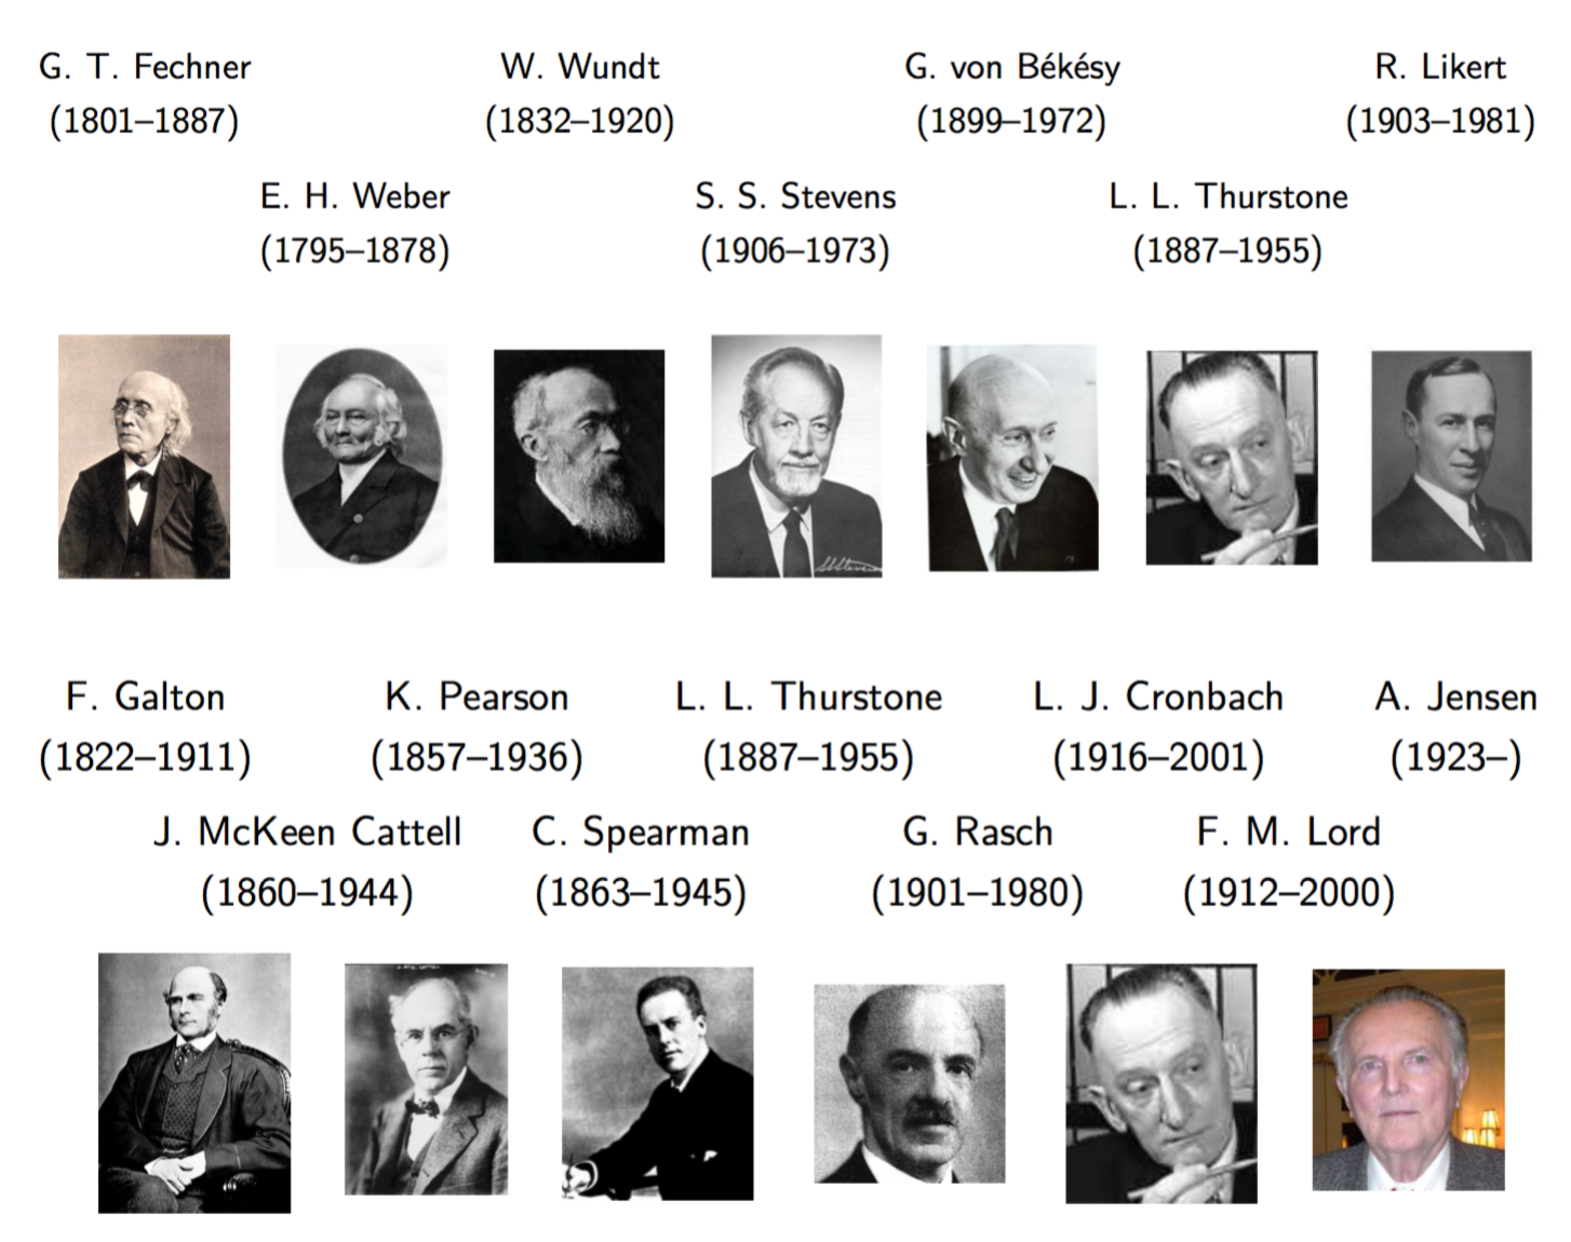
\includegraphics[width=.6\textwidth]{figs/history.eps}}\par}

% ---------------------------------------------------------------Slide-
\foilhead{}

{\centering \fbox{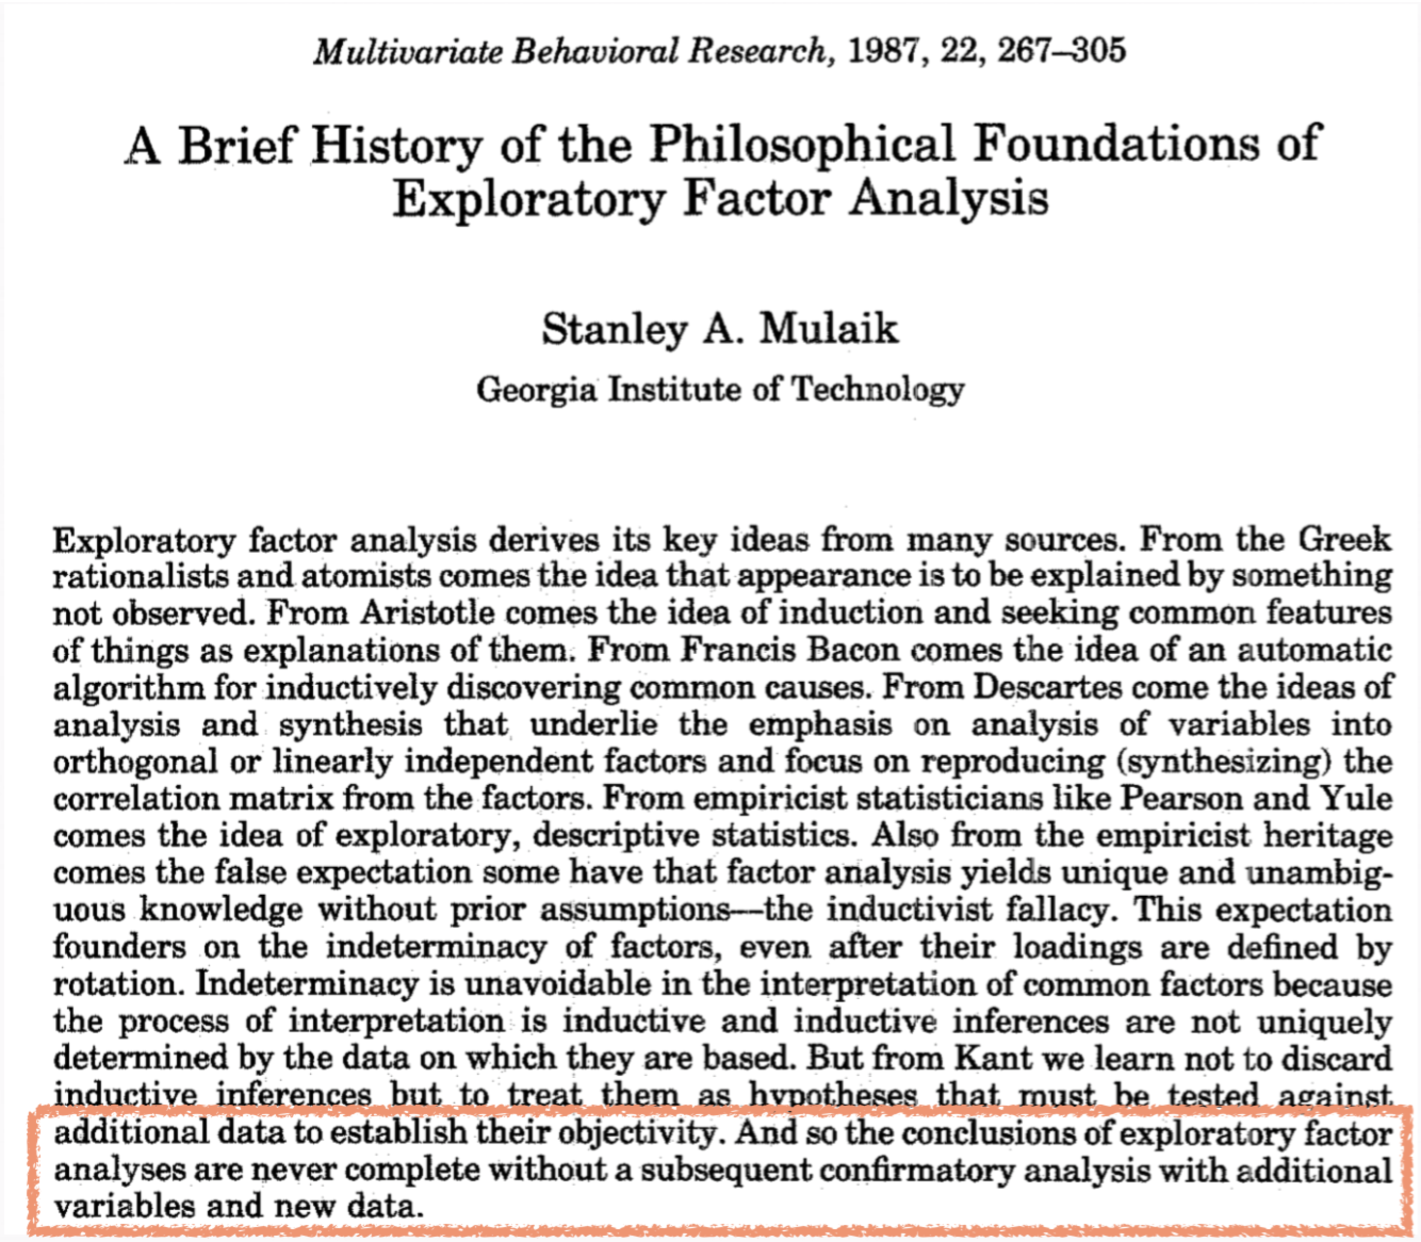
\includegraphics[width=.6\textwidth]{figs/efa.eps}}\par}


% ---------------------------------------------------------------Slide-
\foilhead{ACP et AF}
\hfill $\triangleright$ 01a-scores.pdf

Les composantes $C_i$ ($i=1,\dots,p$) de l'analyse en composantes principales
(ACP) sont construites comme de simples combinaisons linéaires des $p$ variables
d'origine : $C_i=\sum_{j=1}^pw_{ij}\textcolor{Apricot}{x_j}$.

Dans le cadre de l'analyse factorielle, on considère au contraire des
combinaisons linéaires de facteurs\autocite[chap.~ 6]{revelle16} :
\[
\textcolor{Apricot}{x_i}\approx\sum_{j=1}^kw_{ij}\textcolor{CornflowerBlue}{F_j}.
\]


% ---------------------------------------------------------------Slide-
\foilhead{Modèle de Holzinger \& Swineford}

{\centering \fbox{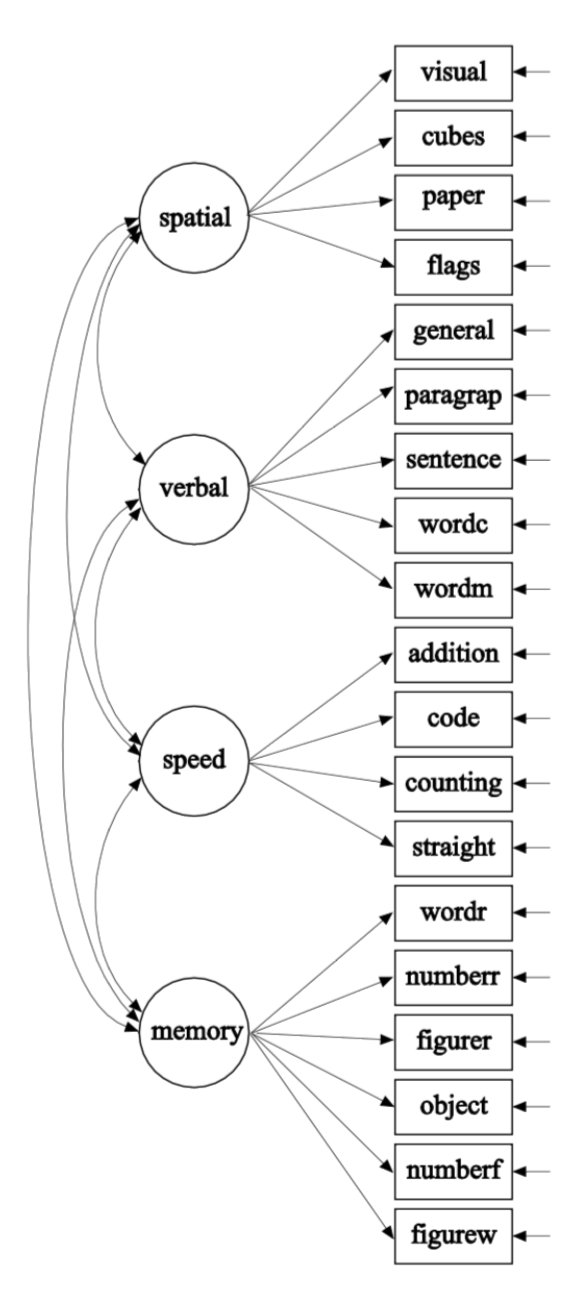
\includegraphics[width=.35\textheight]{figs/HS2.eps}}\par}


% ---------------------------------------------------------------Slide-
\foilhead{Comparaison ACP \emph{versus} AF}

\begin{alltt}
library(psych)
principal(HS[,c("visual","cubes", paper")], \textcolor{Apricot}{nfactors = 3}, 
          rotate = "none")
\end{alltt}
\begin{alltt}\small
Standardized loadings (pattern matrix) based upon correlation matrix
        PC1   PC2   PC3 h2       u2 com
visual 0.77 -0.41  0.48  1  0.0e+00 2.3
cubes  0.70  0.71  0.10  1 -4.4e-16 2.0 \ding{182}
paper  0.80 -0.22 -0.56  1 -6.7e-16 2.0

                       PC1  PC2  PC3
SS loadings           1.72 0.72 0.56
Proportion Var        0.57 0.24 0.19
\end{alltt}

% ---------------------------------------------------------------Slide-
\foilhead{}

\begin{alltt}
fa(HS[,c("visual", "cubes", "paper")], nfactors = 1)
\end{alltt}
\begin{alltt}\small
Standardized loadings (pattern matrix) based upon correlation matrix
        MR1   h2   u2 com
visual 0.62 0.39 0.61   1
cubes  0.48 0.23 0.77   1 \ding{182}
paper  0.71 0.50 0.50   1

                MR1
SS loadings    1.12
Proportion Var 0.37
\end{alltt}

% ---------------------------------------------------------------Slide-
\foilhead{Sélection de modèle}
\begin{itemize}
\item Sélection des variables à inclure : analyse d'items ou hypothèses \emph{a
    priori}
\item Sélection du nombre de facteurs : méthode exploratoire, hypothèses \emph{a
    priori}, analyse parallèle
\item Type de rotation : en fonction des hypothèses théoriques
\item Méthode d'estimation (OLS, ML, WLS et PA)
\item Matrice de corrélation (Pearson, tétra- ou polychorique)  
\item Nombre de sujets nécessaires \autocite{rouquette11}
\end{itemize}


% ---------------------------------------------------------------Slide-
\foilhead{Analyse parallèle}

\begin{alltt}
d <- HS[,7:15]
describe(d)
fa.parallel(d, fm = "pa", fa = "fa", main = "")
\end{alltt}

{\centering 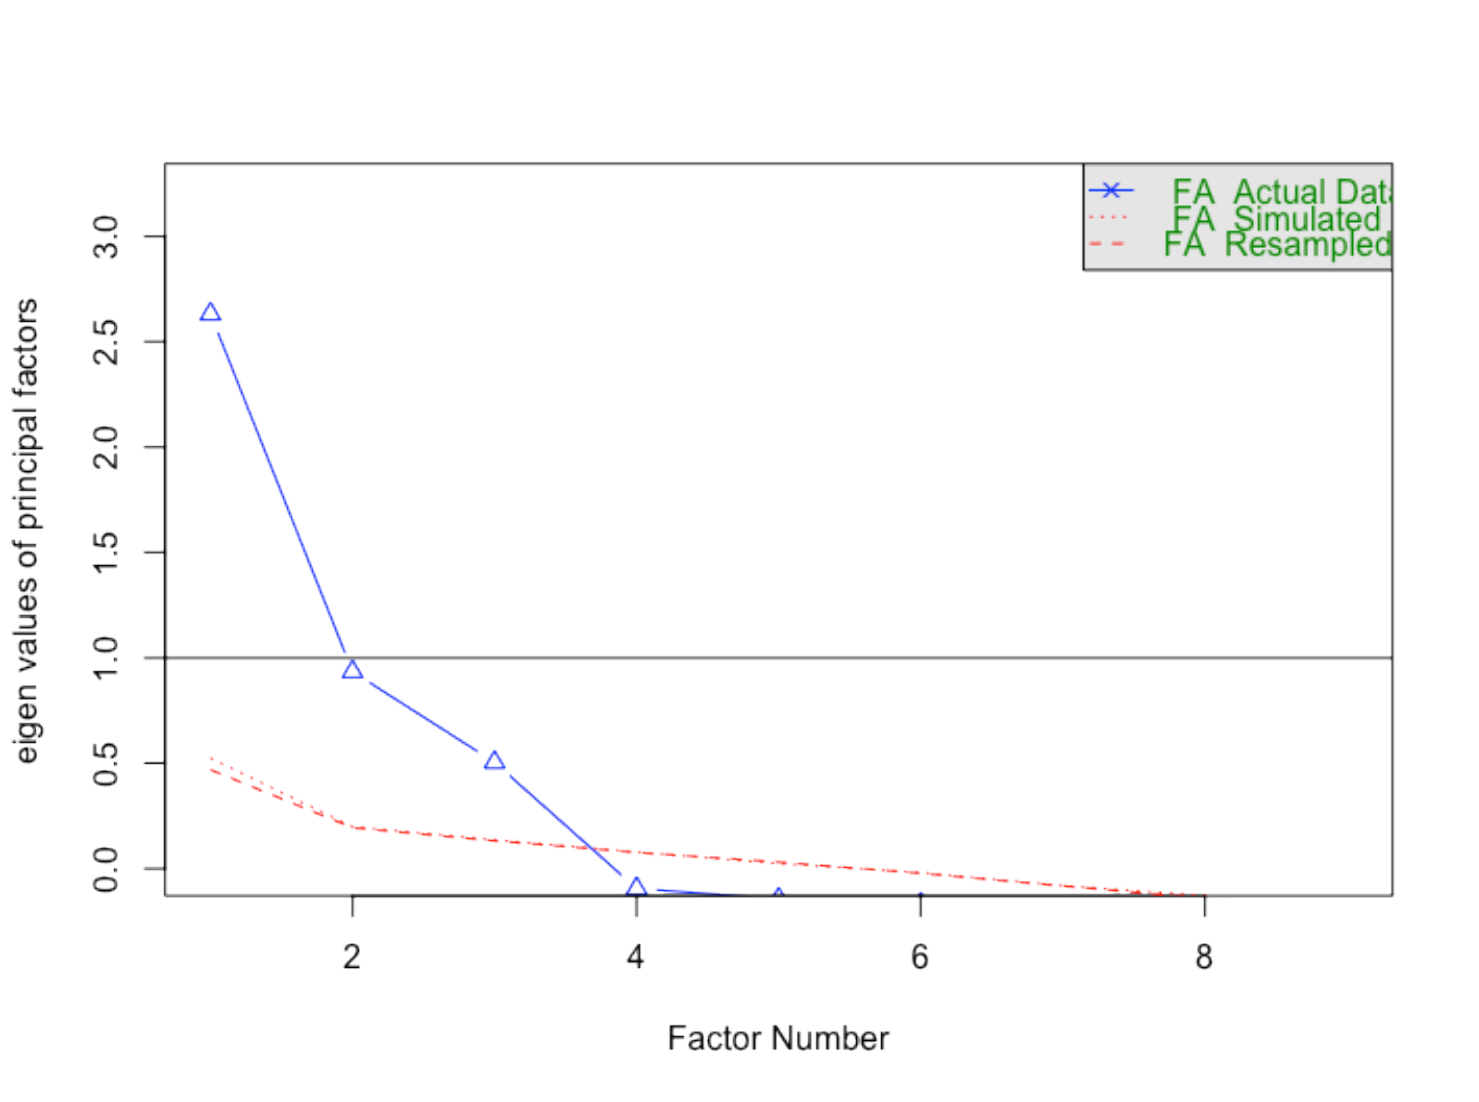
\includegraphics[width=.4\textwidth]{figs/p26.eps}\par}


% ---------------------------------------------------------------Slide-
\foilhead{Solution factorielle à 1 facteur}

{\centering 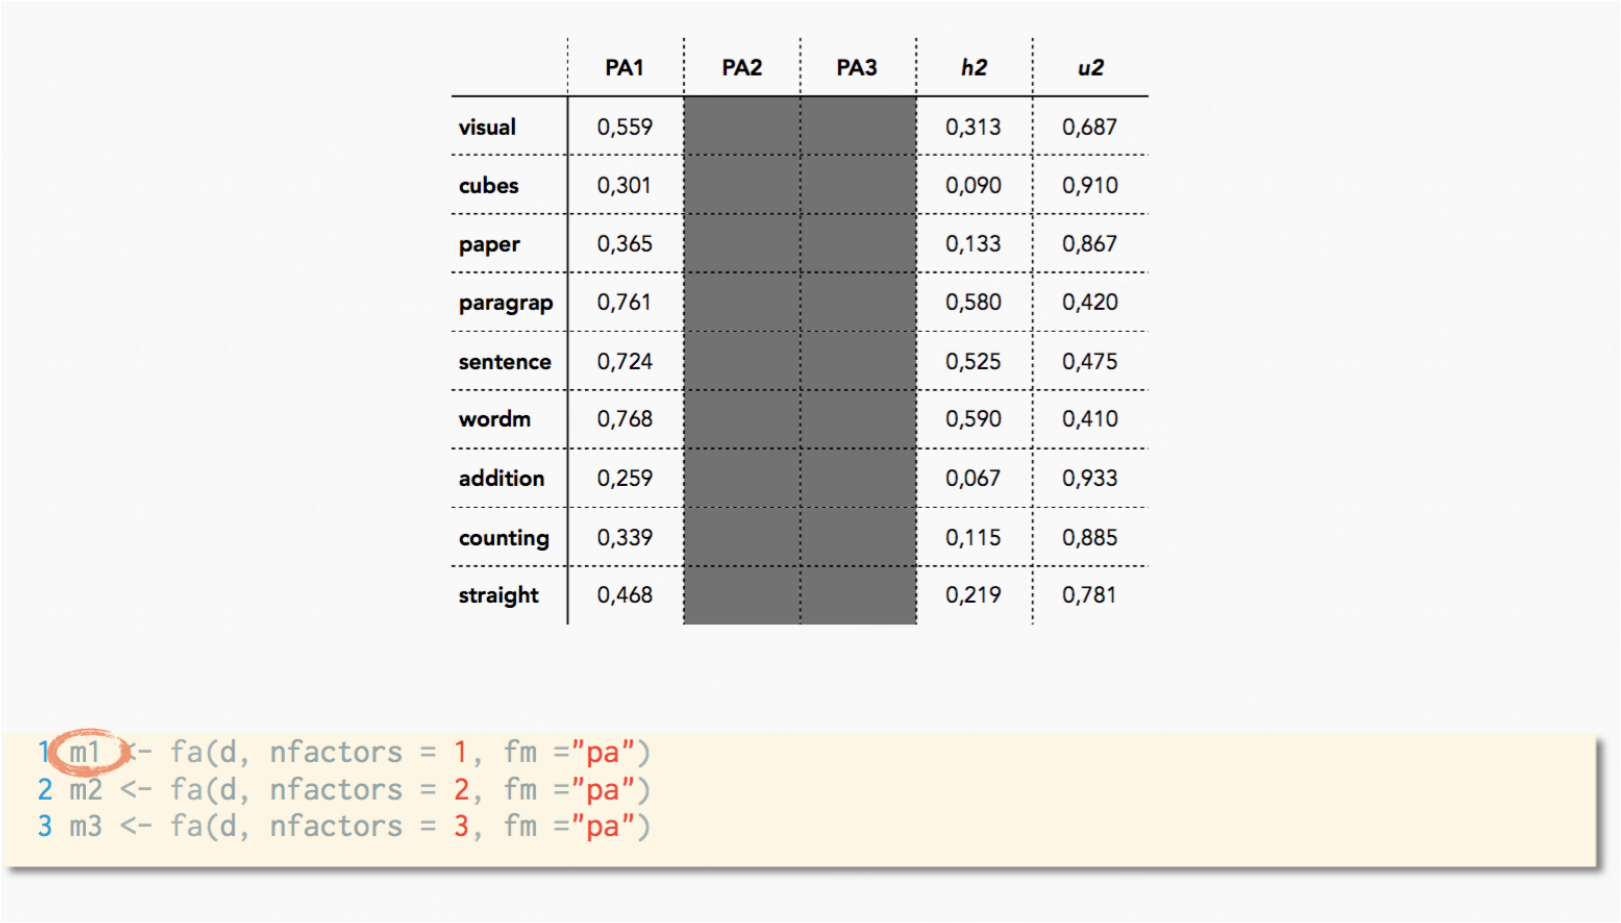
\includegraphics[width=.7\textwidth]{figs/sol1.eps}\par}

% ---------------------------------------------------------------Slide-
\foilhead{Solution factorielle à 2 facteurs}

{\centering 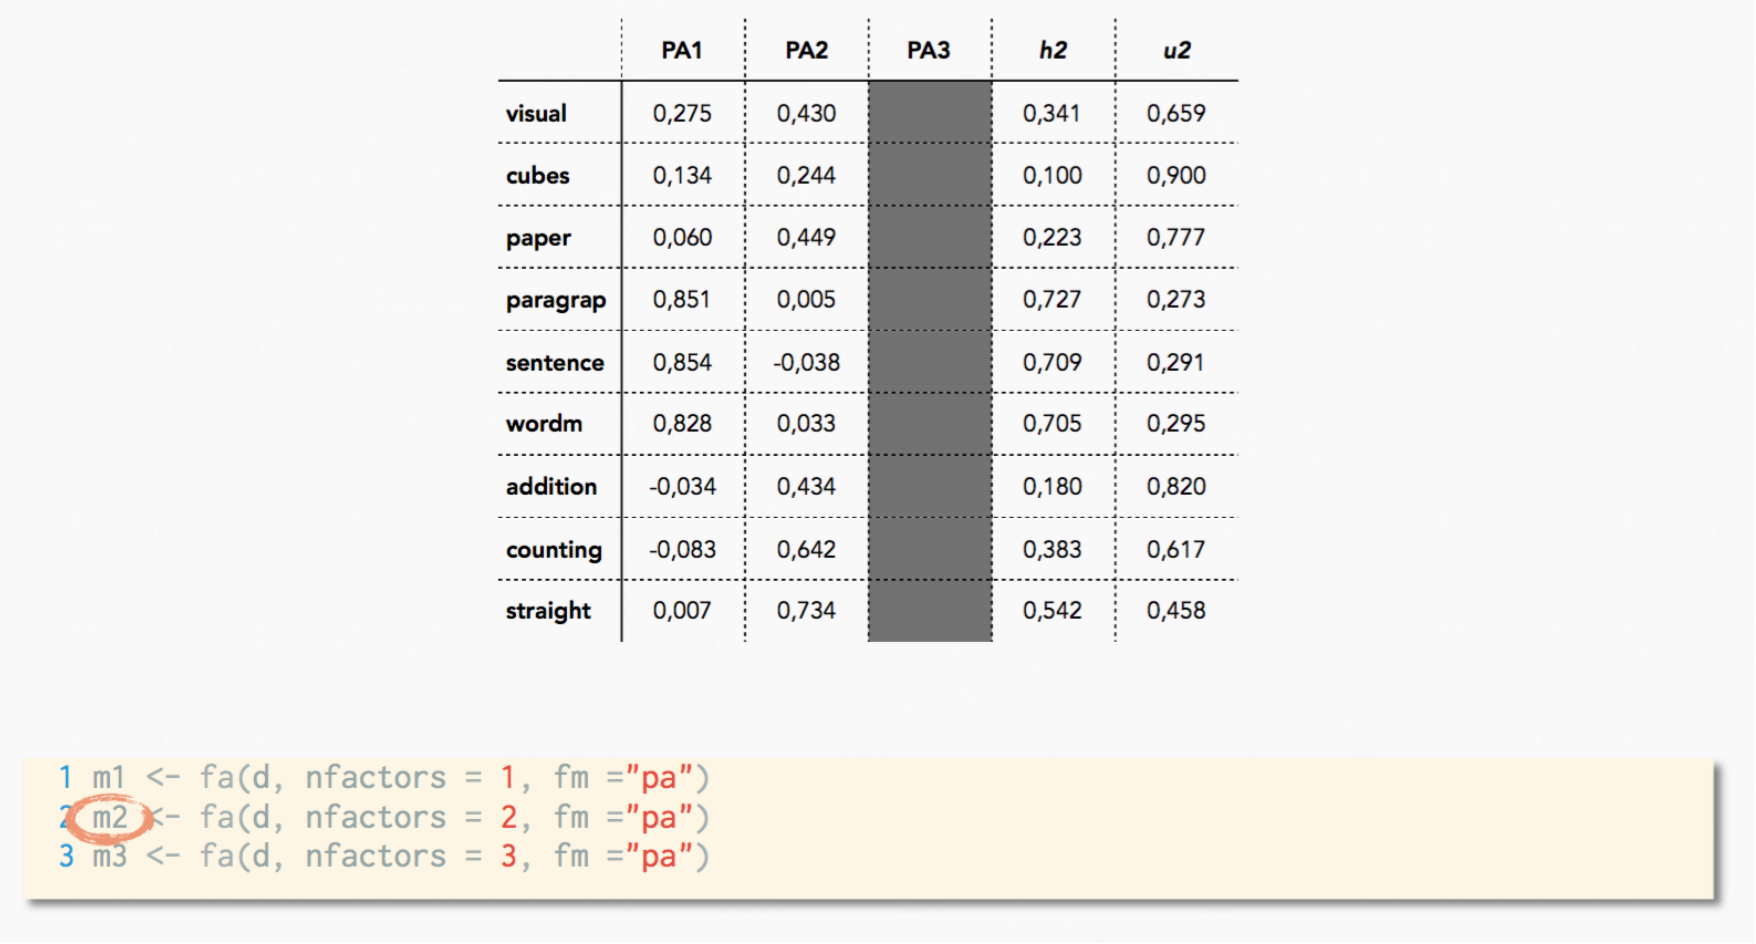
\includegraphics[width=.7\textwidth]{figs/sol2.eps}\par}

% ---------------------------------------------------------------Slide-
\foilhead{Solution factorielle à 3 facteurs}

{\centering 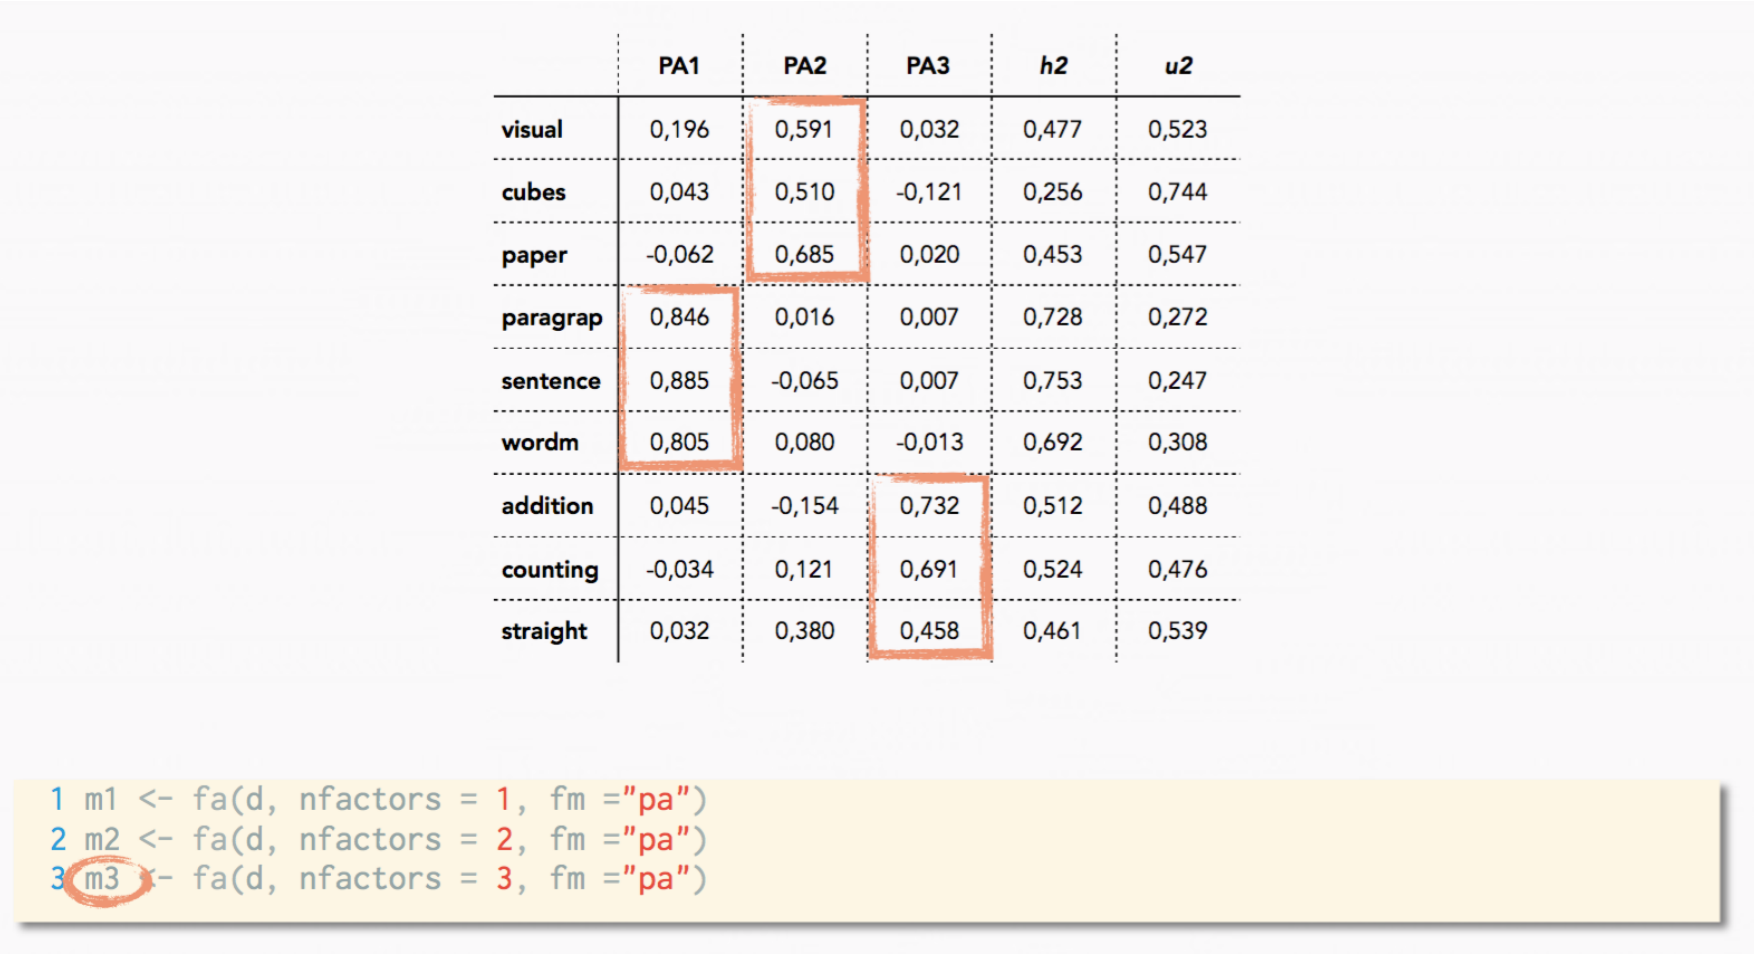
\includegraphics[width=.7\textwidth]{figs/sol3.eps}\par}


% ---------------------------------------------------------------Slide-
\foilhead{Modèles de mesure en analyse factorielle}

{\centering \fbox{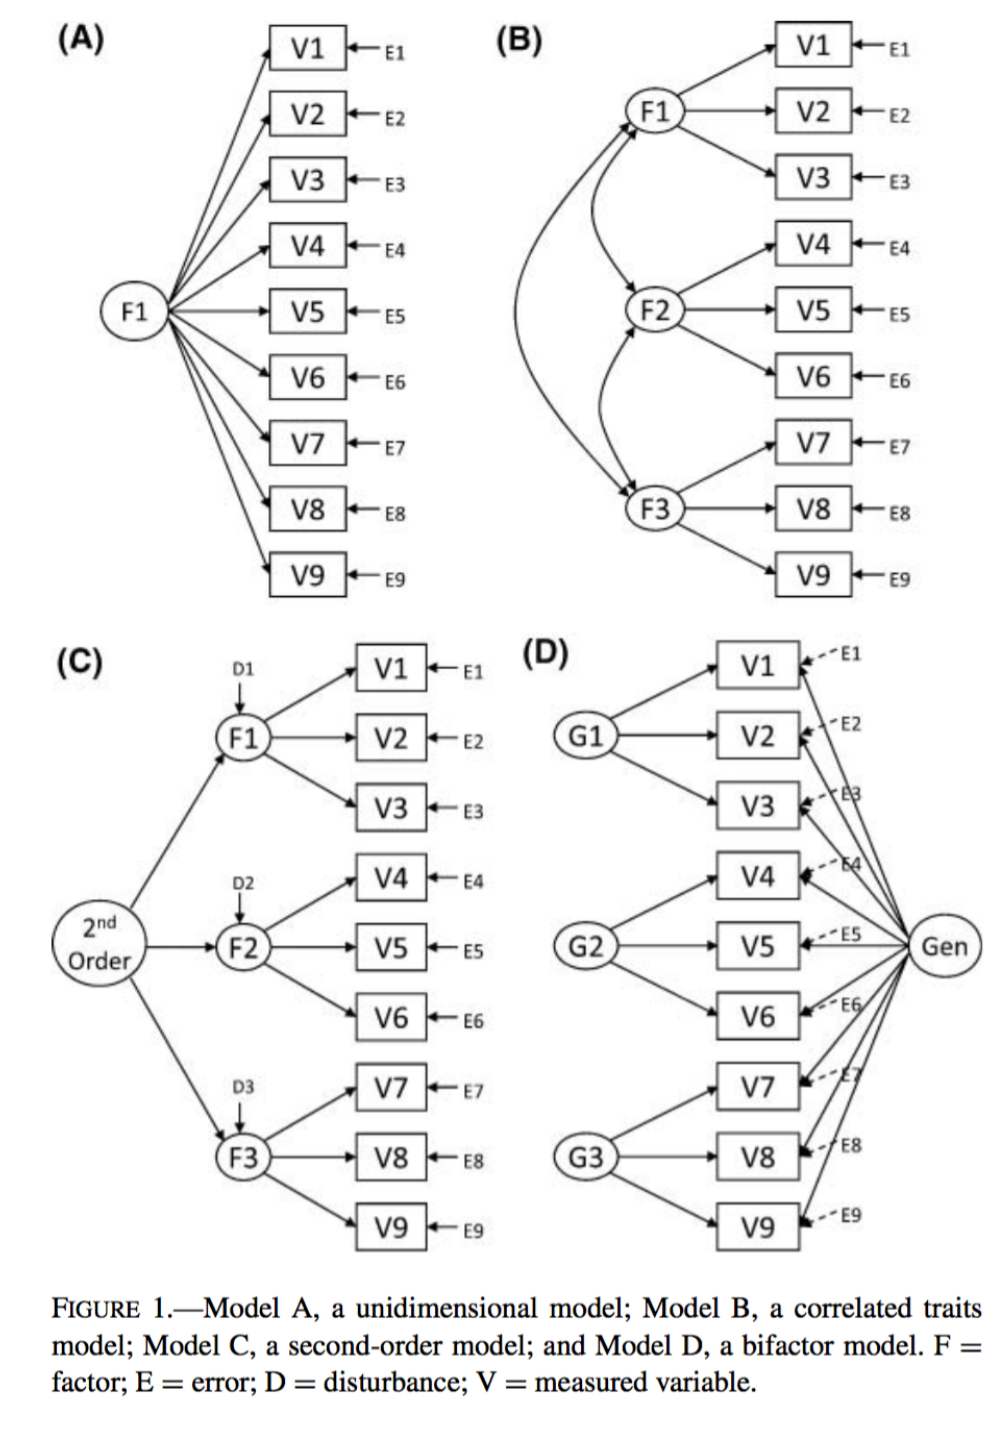
\includegraphics[width=.55\textheight]{figs/models.eps}}\par}


% ---------------------------------------------------------------Slide-
\foilhead{}

Fichier de données et scripts R disponibles à l'adresse suivante :\newline
{\centering \url{https://bitbucket.org/chlalanne/eespe11}\par}
\vfill

\raggedleft \scriptsize -- Typeset with \FoilTeX\ (version 2), Revision \VCRevision

\end{document}
